% \documentclass{beamer}
% \usetheme{Szeged}

% \usepackage{media9}
% \usepackage{graphicx}

% \begin{document}

%-------------------------------------------------------------------------------
%							FOURTH SECTION
%-------------------------------------------------------------------------------
\section{Le problème en 2D}

\subsection{Simulation}
\begin{frame}
    \large
    \centering
    Résultats 2D
\end{frame}

\begin{frame}[fragile]
    \frametitle{Exemple de simulation 2D}
  \begin{center}
    \includemedia[
      width=0.95\linewidth,
      activate=pageopen,
      addresource=Video2D.mp4,
      flashvars={
         source=Video2D.mp4
        &autoPlay=true
      },
      passcontext, % enable VPlayer's right-click menue
    ]{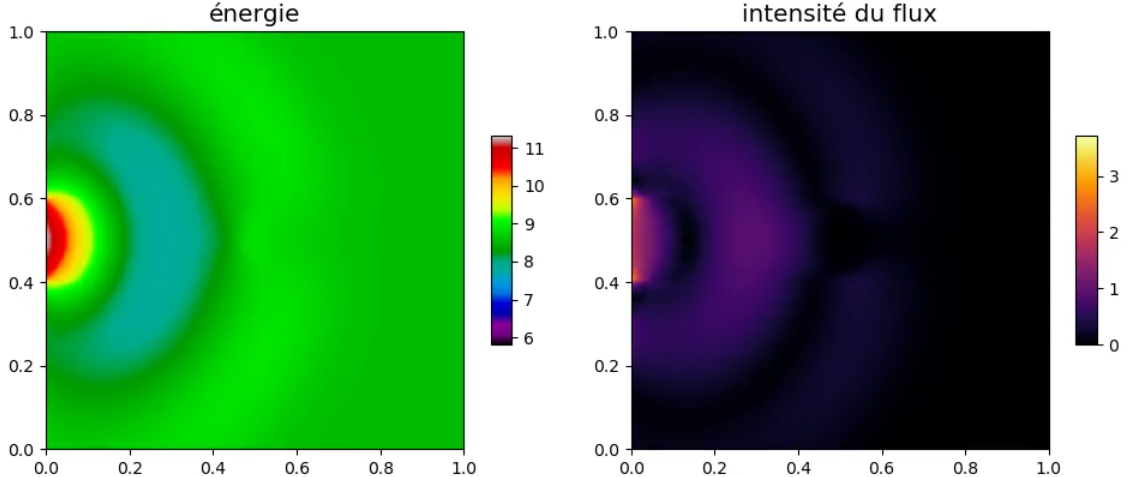
\includegraphics{Thumbnail2D.png}}{VPlayer.swf}%
  \end{center}
\end{frame}

\begin{frame}[fragile]
    \frametitle{Entrées/sorties 2D}

        \begin{figure}
        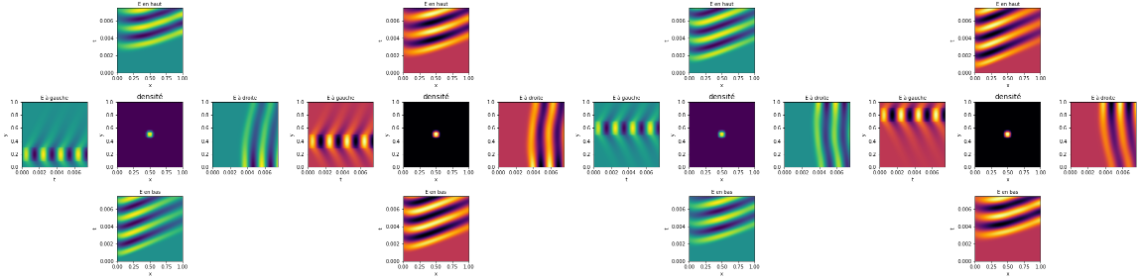
\includegraphics[width=11cm]{EntreeSortie2D}       
        \caption{Une entrée du réseau de neurones et la sortie attendue}
        \end{figure}
        \begin{figure}
        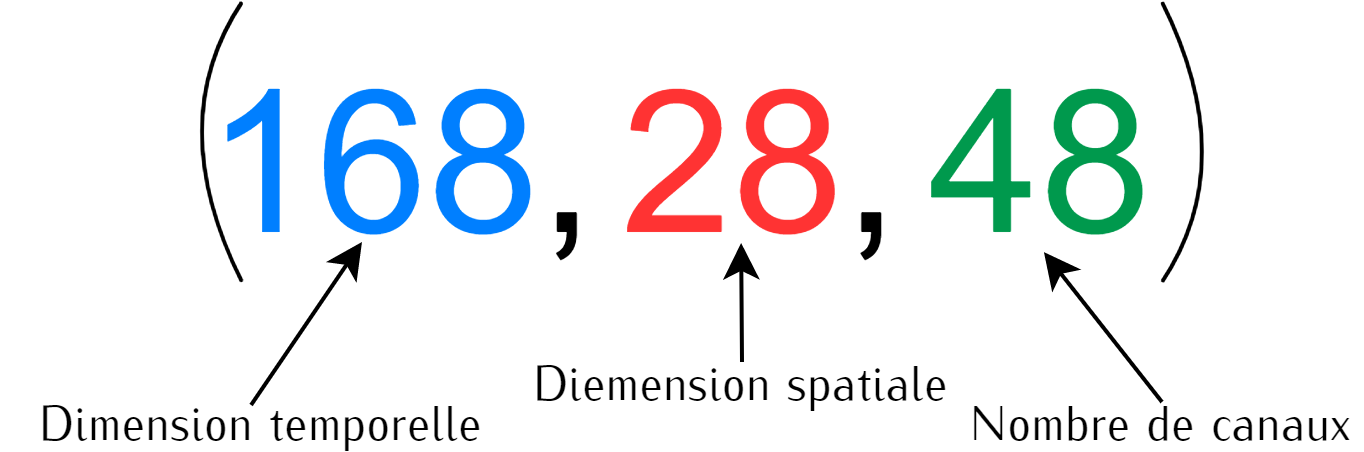
\includegraphics[width=3cm]{Entrees2D}       
        \caption{Taille d'une entrée}
        \end{figure}

\end{frame}

\subsection{Apprentissage}

\begin{frame}[fragile]
    \frametitle{Meilleures/pires prédictions du CNN}

    \begin{columns}
    \begin{column}{0.5\textwidth}
        \begin{figure}
        \includegraphics<1->[width=3cm]{Meilleur2D1}       
        \includegraphics<1->[width=3cm]{Meilleur2D2}       
        \only<1-> {\caption{Les meilleures prédictions}}
        \end{figure}
     \end{column}
     \begin{column}{0.5\textwidth}
        \begin{figure}
        \includegraphics<2>[width=2.5cm]{Pire2D1}       
        \includegraphics<2>[width=2.5cm]{Pire2D2}       
        \includegraphics<2>[width=2.5cm]{Pire2D3}       
        \only<2>{\caption{Les pires prédictions}}
        \end{figure}
     \end{column}
    \end{columns}

\end{frame}

\begin{frame}
    \frametitle{Les scores obtenus en 2D}

    \begin{table}[h!]
        \centering
        \begin{tabular}{l l}
        \toprule
        \textbf{Nom du score} & \textbf{Valeur} \\
        \midrule
        R2 & 98.81 \%\\
        Personnalisé & 93.50 \%\\
        \bottomrule\\
        \end{tabular}
    \end{table}

    \begin{columns}
        \begin{column}{0.333\textwidth}
            \begin{figure}
            \includegraphics<2->[width=2cm]{PositionX2D}       
            \only<2->{\caption{Corrélation des abscisses}}
            \end{figure}
         \end{column}
         \begin{column}{0.333\textwidth}
            \begin{figure}
            \includegraphics<3->[width=2cm]{PositionY2D}       
            \only<3->{\caption{Corrélation des ordonnées}}
            \end{figure}
         \end{column}
         \begin{column}{0.333\textwidth}
            \begin{figure}
            \includegraphics<4->[width=2cm]{Hauteur2D}       
            \only<4->{\caption{Corrélation des hauteurs}}
            \end{figure}
         \end{column}
    \end{columns}

\end{frame}


\begin{frame}
    \frametitle{Conclusion sur la régression 2D}
Détection de toutes les variables :
\begin{itemize}[<+>]
    \item L'abscisse, l'ordonnée, et la hauteur sont relativement bien prédits
    \item La valeur de la densité en dehors du créneau est connue : \textbf{reconstruction complète de la densité du milieu}
\end{itemize}
\end{frame}

\setbeamercovered{invisible}

\begin{frame}
    \frametitle{Classification 2D}
    \begin{columns}
        \begin{column}{0.7\textwidth}
            \begin{figure}
            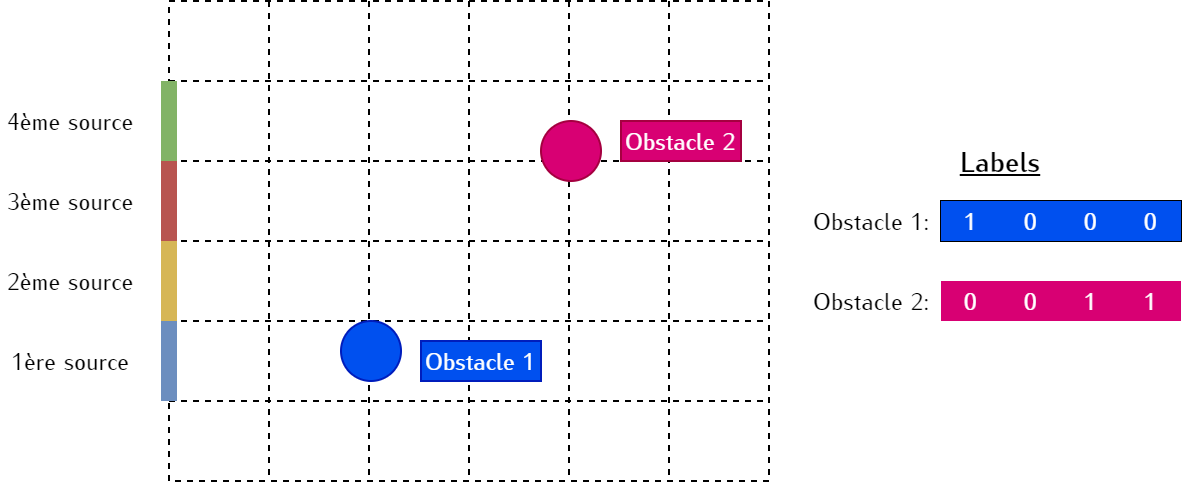
\includegraphics[width=6cm]{Classification}       
            \caption{Labels pour la classification}
            \end{figure}
         \end{column}
         \pause
         \begin{column}{0.3\textwidth}
            \begin{table}[h!]
                \caption{Les scores obtenus}
                \centering
                \begin{tabular}{l l}
                \toprule
                \textbf{Nom} & \textbf{Valeur} \\
                \midrule
                R2 & 98.86 \%\\
                Pers. & 95.45 \%\\
                \bottomrule\\
                \end{tabular}
            \end{table}
         \end{column}
    \end{columns}
\end{frame}

\setbeamercovered{transparent}

% \end{document}
